\section{Operating Charts}
Operating charts describe the modes of operation and the flow of the system without much detail. Figure~\ref{fig:systemFlowchart} shows the system's main flowchart, which depicts how the device goes in and out of each of its operating modes.  A general but brief overview of the different modes of operation follows.

%TODO write paragraph
%When the system is powered up it performs its Boot Sequence, which includes initializing the MCU and all of its peripherals. Once the Boot Sequence has been completed the device will enter Shutdown Mode. In Shutdown Mode the system is operating with very low power and is also listening for a specific RF wake-up signal to further interact with the user. When the device receives the correct wake-up signal it will enter Stand-By Mode. On Stand-By Mode the device establishes a ZigBee connection with the base station. Once connected the user can then select the next operating mode through the proposed GUI. The available selectable operating modes are Diagnostic, Sampling and Data Retrieval modes. The system is not intended for a full power down, but it can occur if the battery is fully depleted, in this case when the device is powered back from such power down it will initialize its boot sequence. Further explanation of the operating modes can be found in each of the modes section.

The following sections contain a more thorough explanation of each of the operating modes mentioned, along with a flowchart of its own to help explain what can be done in each one.
\begin{figure}[H]
	\centering
	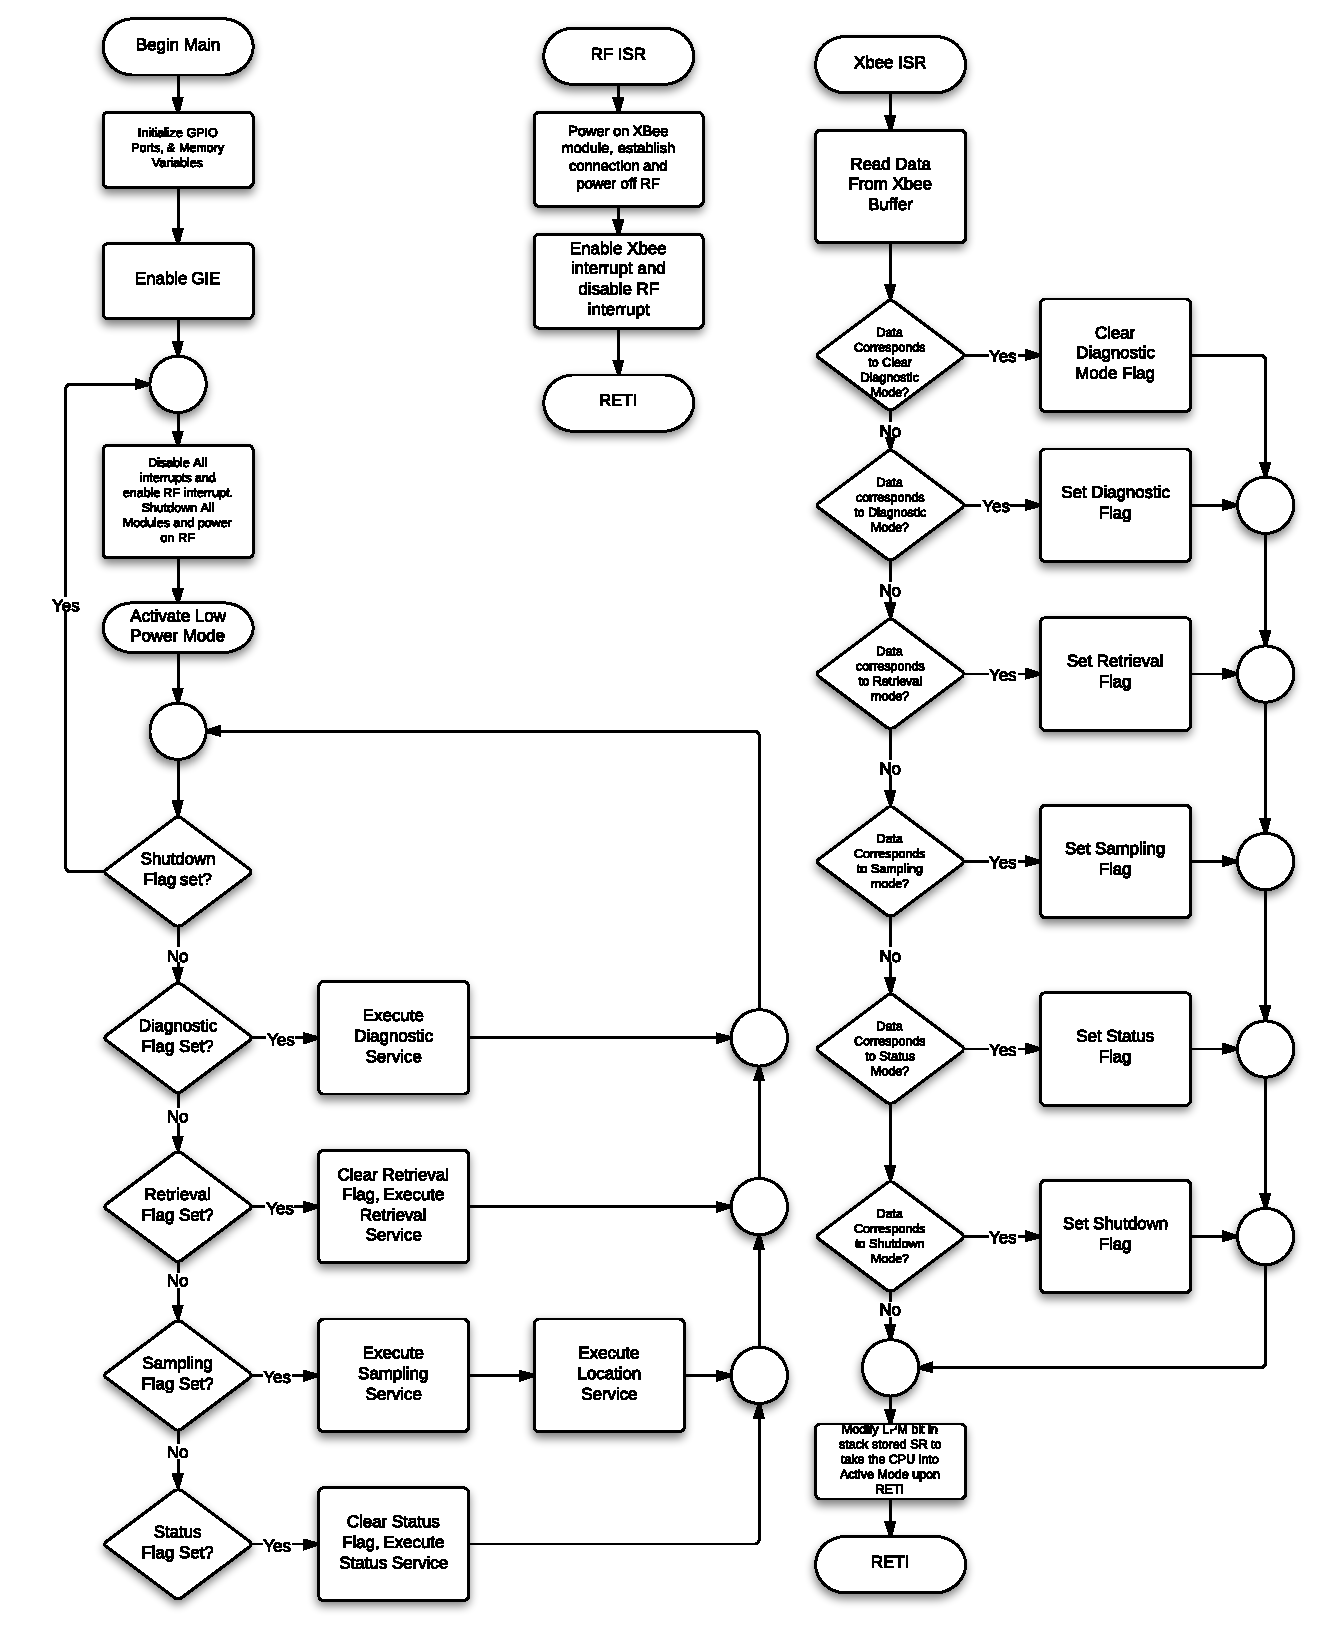
\includegraphics[scale=0.8]{img/SystemFlowchart}
	\caption{System Operating Chart \label{fig:systemFlowchart}}
\end{figure}

\subsection{Diagnostic Event Service}
%TODO fix
On Diagnostic Mode the device maintains communication to the base station and sends real-time information of the different components to the base station, the user can then observe and verify that all components are taking measurements and data can be retrieved through the XBee.
\begin{figure}[H]
	\centering
	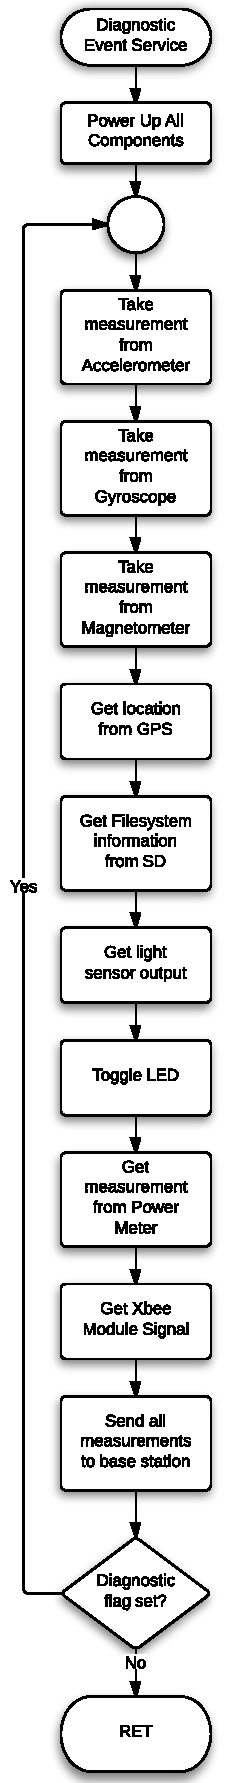
\includegraphics[scale=0.7]{img/DiagnosticEventService}
	\caption{Flowchart for Diagnostic Event Service \label{fig:diagnosticMode}}
\end{figure}

\subsection{Retrieval Event Service}
%TODO fix
Retrieval Mode is the operation mode of the device in which the system transfers the data collected while in Sampling Mode from the SD Card to the base station. Data is transferred trough the established ZigBee connection and once all data has been transferred it is erased from the SD card.
\begin{figure}[H]
	\centering
	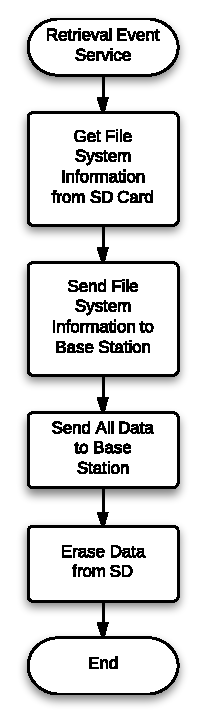
\includegraphics[scale=1.0]{img/RetrievalEventService}
	\caption{Flowchart for Retrieval Event Service \label{fig:retrivalMode}}
\end{figure}


\subsection{Sampling Event Service}
%TODO fix
On Sampling Mode the device captures data from the accelerometer, gyroscope and magnetometer. Data is captured for the duration of the previously specified time and data points are saved in the SD card, each with a time stamp from the time which they were captured.
\begin{figure}[H]
	\centering
	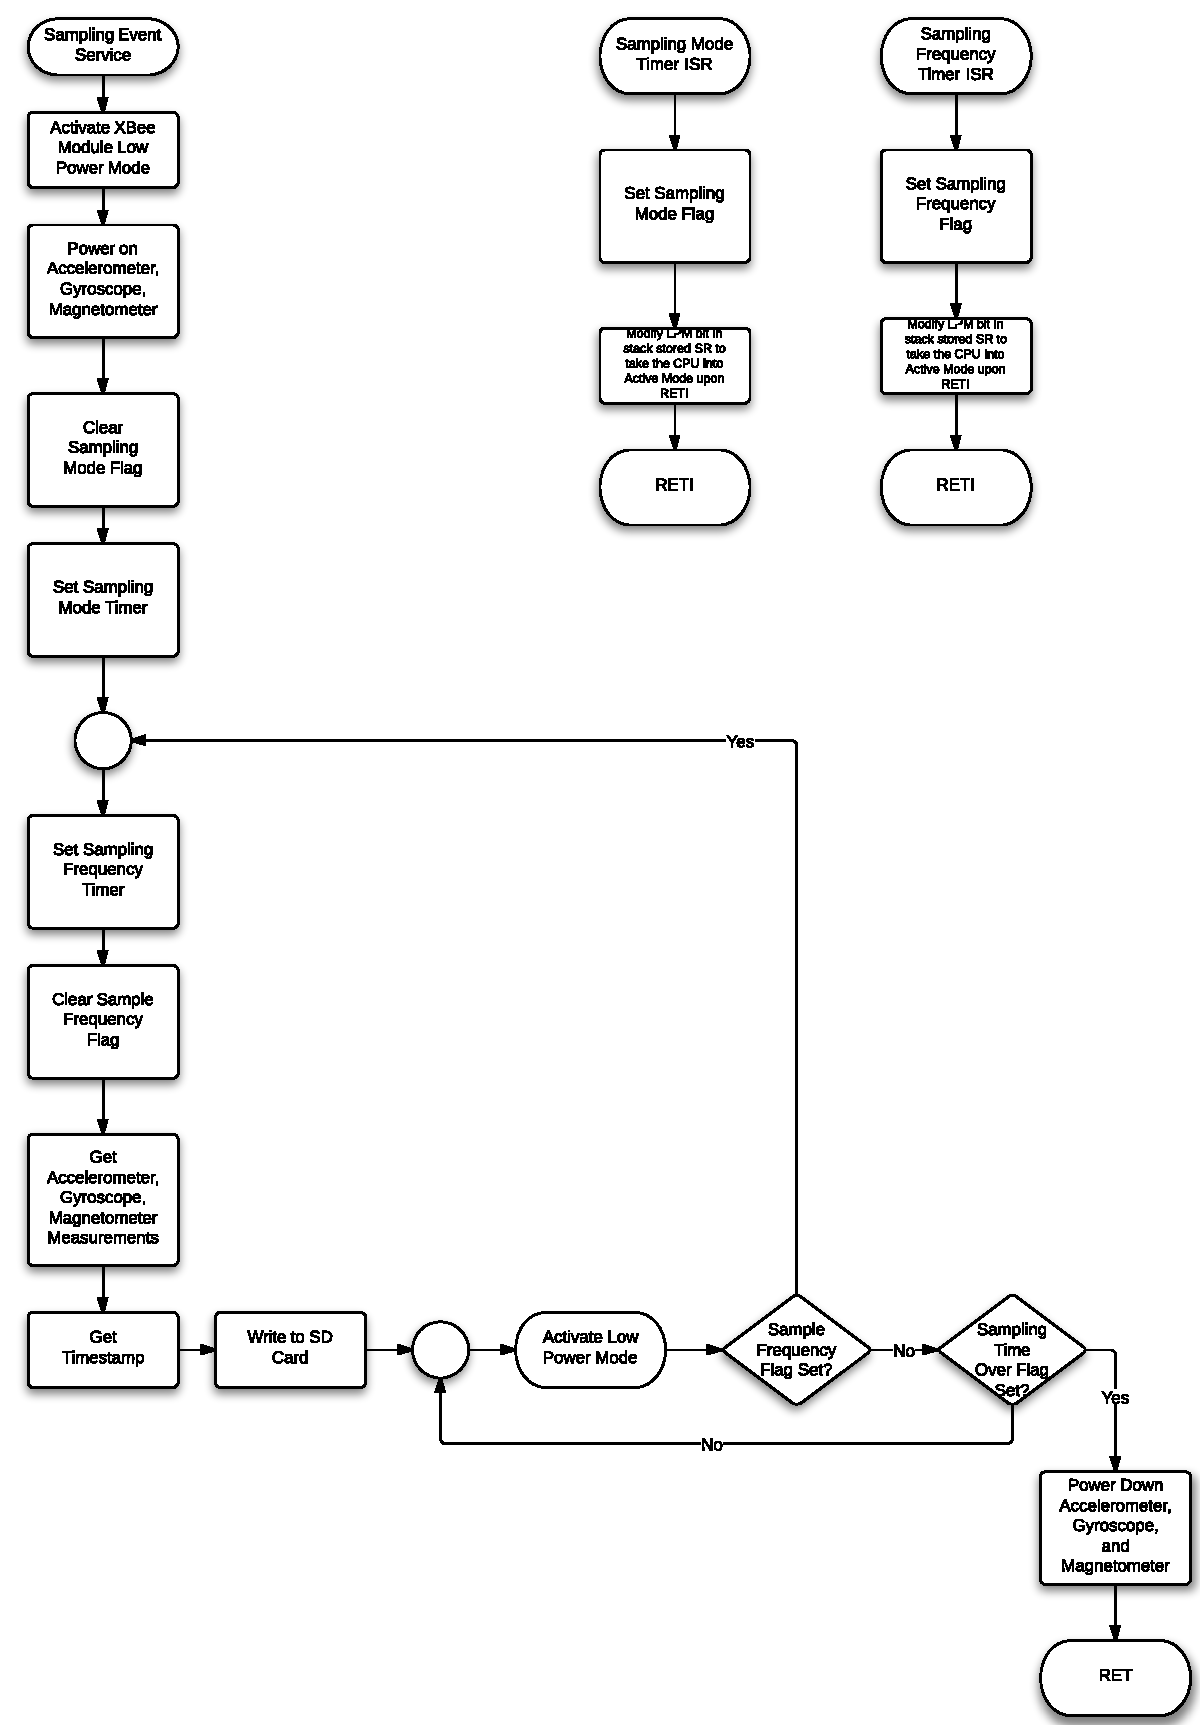
\includegraphics[scale=0.7]{img/SamplingEventService}
	\caption{Flowchart for Sampling Event Service \label{fig:samplingMode}}
\end{figure}

\subsection{Location Event Service}
%TODO fix
On Locate Mode the user is trying find and retrieve the device. The system turns on the XBee Module and the GPS and turns off all other components. The system then proceeds to establishing a ZigBee connection to the base station and get a GPS lock. Once the device gets its location using the GPS Module it will then broadcast the location to the base station through the ZigBee connection. If the on-board light sensor determines that it is dark, i.e.\ an experiment is being conduted when there is little or no sunlight, then a strobe LED will be flashed so as to facilitate the retrieval of the device.
\begin{figure}[H]
	\centering
	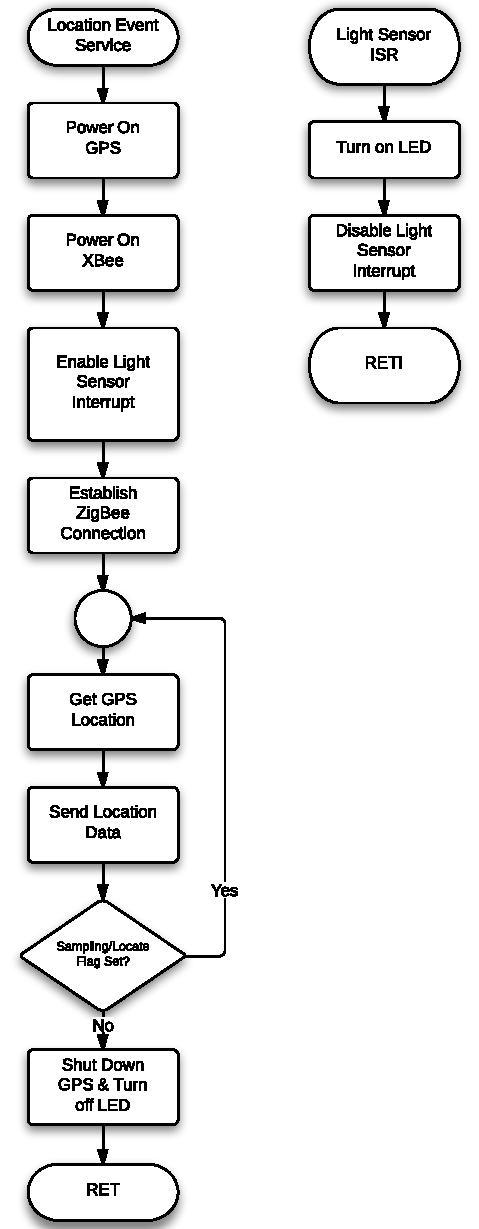
\includegraphics[scale=1.0]{img/LocationEventService}
	\caption{Flowchart for Location Event Service \label{fig:locateMode}}
\end{figure}

\subsection{Status Event Service}
%TODO write explanation paragraph
%On Status mode the system is conserving power with some components turned off while maintaining a ZigBee connection to the base station. At this point, the RTC in the MCU is updated with the current time of the base station. On this mode the system is waiting for user interaction, the device is connected to the base station and simple information is transmitted to the base station's user interface. The transmitted information is battery level and SD card space usage. The system is also waiting for the user to select the next operating mode via the graphical interface on the base station. The user can either test the device with Diagnostic Mode, retrieve its data with Retrieval Mode, or enter Sampling Mode and run an experiment. The components that are awake on this mode are the SD card module and the XBee module and the MCU.
\begin{figure}[H]
	\centering
	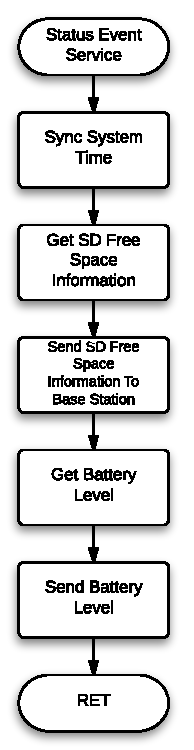
\includegraphics[scale=1.0]{img/StatusEventService}
	\caption{Flowchart for Status Event Service \label{fig:statusMode}}
\end{figure}